%%%%%%%%%%%%%%%%%%%%%%%%%%%%%%%%%%%%%%%%%%%
%
% From a template maintained at https://github.com/jamesrobertlloyd/cbl-tikz-poster
%
% Code near the top should be fairly standard and not need to be changed
%  - except for the document class
% Code lower down is more likely to be customised
%
%%%%%%%%%%%%%%%%%%%%%%%%%%%%%%%%%%%%%%%%%%%

%%%%%%%%%%%%%%%%%%%%%%%%%%%%%%%%%%%%%%%%%%%
%
% Document class
%
% Change this if you want a different size / orientation poster etc
%
%%%%%%%%%%%%%%%%%%%%%%%%%%%%%%%%%%%%%%%%%%%

\documentclass[landscape,a0b,final,a4resizeable]{a0poster}
%\documentclass[portrait,a0b,final,a4resizeable]{a0poster}


\usepackage{multicol}
\usepackage{color}
\usepackage{shadow}
\usepackage{morefloats}
\usepackage{cite}
\usepackage[pdftex]{graphicx}
\usepackage{rotating}
\usepackage{amsmath, amsthm, amssymb, bm}
\usepackage{array}
\usepackage{nth}
\usepackage[square,numbers]{natbib}
\usepackage{booktabs}
%\usepackage{xcolor}

%%%%%%%%%%%%%%%%%%%%%%%%%%%%%%%%%%%%%%%%%%%
%
% TIKZ packages and common definitions
%
% Add extra things as per your tikz needs
%
%%%%%%%%%%%%%%%%%%%%%%%%%%%%%%%%%%%%%%%%%%%

\usepackage{../common/picins}
\usepackage{tikz}
\usetikzlibrary{shapes.geometric,arrows,chains,matrix,positioning,scopes,calc}
\tikzstyle{mybox} = [draw=white, rectangle]

%%%%%%%%%%%%%%%%%%%%%%%%%%%%%%%%%%%%%%%%%%%
%
% myfig
%
% \myfig - replacement for \figure
% necessary, since in multicol-environment 
% \figure won't work        
%                 
%%%%%%%%%%%%%%%%%%%%%%%%%%%%%%%%%%%%%%%%%%%

\newcommand{\myfig}[3][0]{
\begin{center}
  \vspace{1.5cm}
  \includegraphics[width=#3\hsize,angle=#1]{#2}
  \nobreak\medskip
\end{center}}

%%%%%%%%%%%%%%%%%%%%%%%%%%%%%%%%%%%%%%%%%%%
%
% mycaption                
%
% \mycaption - replacement for \caption
% necessary, since in multicol-environment \figure and
% therefore \caption won't work
%
%%%%%%%%%%%%%%%%%%%%%%%%%%%%%%%%%%%%%%%%%%%

%\newcounter{figure}
\setcounter{figure}{1}
\newcommand{\mycaption}[1]{
  \vspace{0.5cm}
  \begin{quote}
    {{\sc Figure} \arabic{figure}: #1}
  \end{quote}
  \vspace{1cm}
  \stepcounter{figure}
}

%%%%%%%%%%%%%%%%%%%%%%%%%%%%%%%%%%%%%%%%%%%
%
% Some standard colours
%
%%%%%%%%%%%%%%%%%%%%%%%%%%%%%%%%%%%%%%%%%%%

\definecolor{camlightblue}{rgb}{0.601 , 0.8, 1}
\definecolor{camdarkblue}{rgb}{0, 0.203, 0.402}
\definecolor{camred}{rgb}{1, 0.203, 0}
\definecolor{camyellow}{rgb}{1, 0.8, 0}
\definecolor{lightblue}{rgb}{0, 0, 0.80}
\definecolor{white}{rgb}{1, 1, 1}
\definecolor{whiteblue}{rgb}{0.80, 0.80, 1}

%%%%%%%%%%%%%%%%%%%%%%%%%%%%%%%%%%%%%%%%%%%
%
% Some look and feel definitions
%
%%%%%%%%%%%%%%%%%%%%%%%%%%%%%%%%%%%%%%%%%%%

\setlength{\columnsep}{0.03\textwidth}
\setlength{\columnseprule}{0.0018\textwidth}
\setlength{\parindent}{0.0cm}

%%%%%%%%%%%%%%%%%%%%%%%%%%%%%%%%%%%%%%%%%%%
%
% \mysection - replacement for \section*
% 
% Puts a pretty box around some text
% TODO - any other thoughts for what this box should look like
%
%%%%%%%%%%%%%%%%%%%%%%%%%%%%%%%%%%%%%%%%%%%

\tikzstyle{mysection} = [rectangle, 
									draw=none, 
									shade, 
									outer color=camlightblue!30,
									inner color=camlightblue!30,
									text width=0.965\columnwidth,
									text centered,
									rounded corners=20pt,
									minimum height=0.11\columnwidth]

\newcommand{\mysection}[1]
{
\begin{center}
  \begin{tikzpicture}
    \node[mysection] {\sffamily\bfseries\LARGE#1};
  \end{tikzpicture}
\end{center}
}

%%%%%%%%%%%%%%%%%%%%%%%%%%%%%%%%%%%%%%%%%%%
%
% Set the font
%
% TODO - Not sure what a canonical choice is - feel free to modify
%
%%%%%%%%%%%%%%%%%%%%%%%%%%%%%%%%%%%%%%%%%%%

\renewcommand{\familydefault}{cmss}
\sffamily

%%%%%%%%%%%%%%%%%%%%%%%%%%%%%%%%%%%%%%%%%%%
%
% Poster environment
%
% Centres everything and can be used to define the width of the content
%
%%%%%%%%%%%%%%%%%%%%%%%%%%%%%%%%%%%%%%%%%%%

\newenvironment{poster}{
  \begin{center}
  \begin{minipage}[c]{0.96\textwidth}
}{
  \end{minipage} 
  \end{center}
}

%%%%%%%%%%%%%%%%%%%%%%%%%%%%%%%%%%%%%%%%%%%
%
% This is probably a good place to put content specific packages and definitions
%
%%%%%%%%%%%%%%%%%%%%%%%%%%%%%%%%%%%%%%%%%%%

%\usepackage{preamble}
\usepackage{tabularx}

\def\newarrow{\mbox{\begin{tikzpicture}
             \useasboundingbox{(-3pt,-4.5pt) rectangle (19pt,1pt)};
             \draw[->] (0,-0.07)--(17pt,-0.07);\end{tikzpicture}}}
             
\usepackage[autostyle]{csquotes}  

%%%%%%%%%%%%%%%%%%%%%%%%%%%%%%%%%%%%%%%%%%%
%
% The document environment starts here
%
%%%%%%%%%%%%%%%%%%%%%%%%%%%%%%%%%%%%%%%%%%%

\begin{document}

%%%%%%%%%%%%%%%%%%%%%%%%%%%%%%%%%%%%%%%%%%%
%
% Begin the poster environment - centres things and potentially changes the width
%
%%%%%%%%%%%%%%%%%%%%%%%%%%%%%%%%%%%%%%%%%%%

\begin{poster}

%%%%%%%%%%%%%%%%%%%%%%%%%%%%%%%%%%%%%%%%%%%
%
% Potentially add some space at the top of the poster
%
%%%%%%%%%%%%%%%%%%%%%%%%%%%%%%%%%%%%%%%%%%%

\vspace{0\baselineskip}

%%%%%%%%%%%%%%%%%%%%%%%%%%%%%%%%%%%%%%%%%%%
%
% Draw the header as a TIKZ picture
%
% Using TIKZ to allow for easy alignment
%
%%%%%%%%%%%%%%%%%%%%%%%%%%%%%%%%%%%%%%%%%%%

\begin{center}
\begin{tikzpicture}[x=0.5\textwidth]
    % Dummy nodes at edges for spacing
    % TODO - a better way?
    \node at (+1, 0) {};    
    \node at (-1, 0) {};
    % Set the size of the badges
    \def \badgeheight {0.08\textwidth}
    % Title text
    \node[inner sep=0,text width=0.7\textwidth,text centered,font=\Huge] (Title) at (0,0) 
    {
      {\sffamily \Huge \textbf{Statistical Model Criticism using Kernel Two Sample Tests}}\\
      {\huge\sffamily James Robert Lloyd and Zoubin Ghahramani}\\
      \vspace{-0.3\baselineskip}
      {\large\sffamily Department of Engineering, University of Cambridge, UK}
    };
    % Cambridge badge
    \node [mybox] (Cambridge Badge) at (-0.9, 0) {
        \includegraphics[height=\badgeheight]{../badges/cam-crest-and-text.pdf}
    };
    % CBL badge
    \node [mybox] (CBL Badge) at (+0.9, 0) {
        
\includegraphics[height=\badgeheight]{../badges/cbl-badge-cropped.png}
    };
    % MIT badge
    %\node [mybox] (MIT Badge) at (+0.825, 0) {
    %    
\includegraphics[height=\badgeheight]{../badges/MIT2.jpg}
    %};
    % QR code
    %\node [mybox] (QR code) at (-0.95, 0) {
    %    
\includegraphics[height=\badgeheight]{../badges/QR.png}
    %};
\end{tikzpicture}
\end{center}

%%%%%%%%%%%%%%%%%%%%%%%%%%%%%%%%%%%%%%%%%%%
%
% Spacing between title and main body
%
%%%%%%%%%%%%%%%%%%%%%%%%%%%%%%%%%%%%%%%%%%%

\vspace{1\baselineskip}

%%%%%%%%%%%%%%%%%%%%%%%%%%%%%%%%%%%%%%%%%%%
%
% Columns environment
%
%%%%%%%%%%%%%%%%%%%%%%%%%%%%%%%%%%%%%%%%%%%

\begin{multicols}{3}

%%%%%%%%%%%%%%%%%%%%%%%%%%%%%%%%%%%%%%%%%%%
%
% Start of content
%
%%%%%%%%%%%%%%%%%%%%%%%%%%%%%%%%%%%%%%%%%%%

\large

\mysection{Summary of paper}

\vspace{1\baselineskip}

\begin{itemize}
  \item We think that model criticism is very important but underrepresented in much of the machine learning literature
  \vspace{0.5\baselineskip}
  \item We investigated the application of a kernel hypothesis test to model criticism and give examples of its usage
  \vspace{0.5\baselineskip}
  \item But most importantly we would like more people to be mindful of the benefits of model criticism. Ask yourself, \textbf{Do you know how the model you are currently working with most misrepresents the data it is attempting to model?}
\end{itemize}

\vspace{1\baselineskip}

\mysection{What is model criticism?}

\vspace{1\baselineskip}

Simplifying drastically, model criticism asks the question, ``is my model wrong?''.
For example, consider this one dimensional data represented by a histogram.
Would this data be fit well by a normal distribution?

\begin{center}
  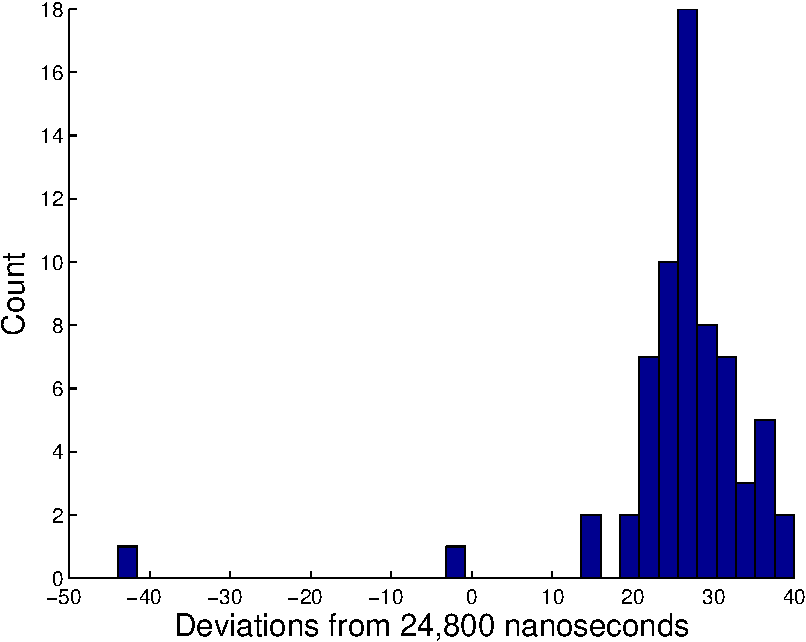
\includegraphics[width=0.48\columnwidth]{../figures/newcomb_hist}
\end{center}

Answer: Of course not, there are gross outliers.

\vspace{1\baselineskip}

Simplifying slightly less, many model criticism methods are composed of:

\vspace{1\baselineskip}

\begin{itemize}
  \item A null hypothesis in the form of a model or models of data e.g.
  \begin{itemize}
    \item A class of models e.g.\ all linear regression models with Gaussian noise
    \item A particular model e.g.\ a neural network after training
    \item A distribution over models e.g.\ prior or posterior distributions
  \end{itemize}
  \item A statistic to measure how extreme a collection of data is e.g.
  \begin{itemize}
    \item The largest distance between any two data points
    \item The minimum value of the likelihood of individual data points under a model (i.e.\ an outlier measure)
  \end{itemize}
  \item A method to perform an alternative free hypothesis test using this statistic and null hypothesis
\end{itemize}

\vspace{1\baselineskip}

The result of model criticism is then a measure of how surprising the data is, viewed through some statistic, under the assumption of some model or class of models.
The question that motivated this research was, \textbf{How do we choose the statistic by which to measure how surprising our data is?}

\vspace{1\baselineskip}

\newpage

\mysection{Why do we need model criticism?}

Answer: Science!

%\vspace{1\baselineskip}

%\begin{quotation}
%``A man in daily muddy contact with field experiments could not be expected to have much faith in any direct assumption of independently distributed normal errors''
%\end{quotation}

%\vspace{1\baselineskip}

%But perhaps more importantly, vigorous criticism is an essential part of the scientific method

%\item \dots and that can lead to false conclusions\dots

%\begin{quotation}
%``We were seeing things that were 25-standard deviation moves, several 
%days in a row'
%\end{quotation}

\begin{center}
  \large
  \tikzstyle{block} = [rectangle, draw, fill=blue!20, 
                       text width=0.2\columnwidth, text centered, rounded corners, minimum height=3em]
  \tikzstyle{line} = [draw, -latex', line width=10pt]
  \tikzstyle{thin line} = [draw, -latex', line width=5pt]
  \tikzstyle{cloud} = [draw, ellipse,fill=red!20,minimum height=2em]
    
  \begin{tikzpicture}[node distance = 0.3\columnwidth]
    % Place nodes
    \node [block] at (0, 0) (hypothesis) {Hypothesis generation};
    \node [block] at (0.4\columnwidth, 0) (infer) {Deduction and inference};
    %\node [cloud] at (0.4\columnwidth, -0.2\columnwidth) (apply) {Application};
    %\node [cloud] at (0.4\columnwidth, +0.2\columnwidth) (data) {Data};
    \node [block] at (0.8\columnwidth, 0) (criticise) {Evaluation and \bf{criticism}};
    % Draw edges
    \path [line] (hypothesis.east) -- (infer.west);
    \path [line] (infer.east) -- (criticise.west);
    %\path [thin line] (infer.south) -- (apply.north);
    %\path [thin line] (data.south) -- (infer.north);
    %\path [thin line] (data.south east) -- (criticise.north west);
    %\path [thin line] (hypothesis.north east) -- (data.south west);
    %\path [thin line] (criticise.south west) -- (apply.north east);
    \draw[->, , line width=10pt] (criticise.south) .. controls (0.6\columnwidth,-0.2\columnwidth) and (0.2\columnwidth,-0.2\columnwidth) .. (hypothesis.south);
  \end{tikzpicture}
\end{center}

%\vspace{1\baselineskip}

Vigorous criticism is an essential part of the scientific method.
Machine learning has been focused on model performance i.e.\ evaluation, which provides little information on \textbf{how to improve} a model.

%\vspace{1\baselineskip}

\mysection{Kernel two sample tests}

%\vspace{1\baselineskip}

Suppose we have samples ${X = (x_i)_{i=1\ldots m}}$ and ${Y = (y_i)_{i=1\ldots n}}$ drawn iid.\ from distributions $p$ and $q$ respectively.
The two sample problem asks if $p = q$.
A way of answering the two sample problem is to consider maximum mean discrepancy (MMD) statistics
\vspace{-1\baselineskip}
\begin{equation*}
\textrm{MMD}(\mathcal{F},p,q) = \sup_{f \in \mathcal{F}}(\mathbb{E}_{x\sim p}[f(x)] - \mathbb{E}_{y\sim q}[f(y)])
\label{eq:MMD}
\vspace{-1\baselineskip}
\end{equation*}
where $\mathcal{F}$ is a set of functions.
When $\mathcal{F}$ is a reproducing kernel Hilbert space (RKHS) the function attaining the supremum (called the witness function) and the value of the MMD can be estimated from finite samples.

%\vspace{1\baselineskip}

\mysection{Application to model criticism}

%\vspace{1\baselineskip}

We return to the central question \textbf{How do we choose the statistic by which to measure how surprising our data is?}
Kernel two sample tests are of interest since they are defined as a maximisation over a large class of statistics; in a weak sense the statistic is selected automatically.
Moreover we can use this statistic to identify where a model and data disagree most.

%\begin{tabularx}{0.96\columnwidth}{X X}

\setlength{\columnseprule}{0\textwidth}
\begin{multicols}{2}

Returning to our histogram data, we fit a normal distribution to it (red line) and then performed a kernel two sample test, resulting in the witness function shown in dashed green.
The witness function peaks indicate where there is less data than expected; the troughs where there is more.

\newpage

\begin{center}
  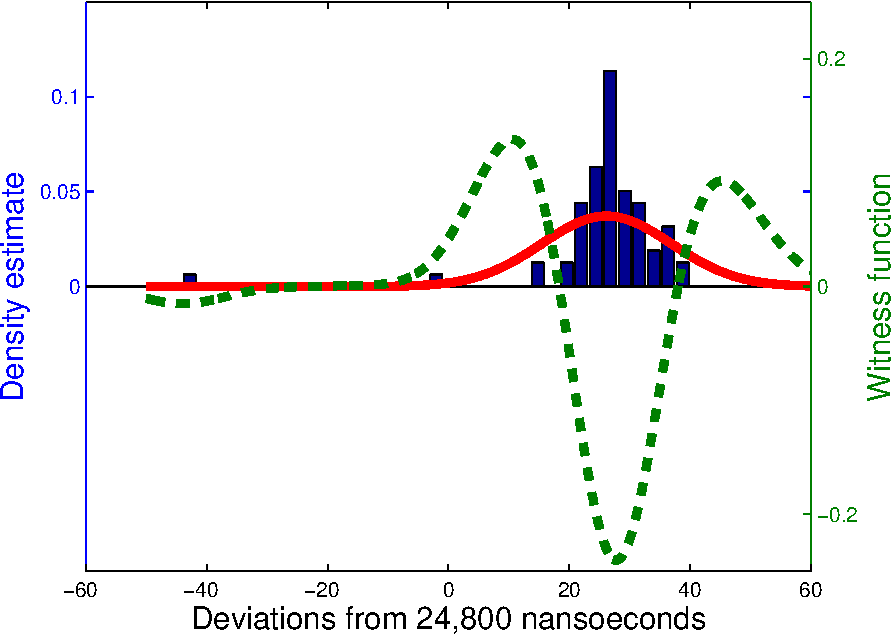
\includegraphics[width=0.96\columnwidth]{../figures/newcomb_witness_1}
\end{center}

\end{multicols}

Note that the main discrepancies between model and data (by this measure) are not near the outlier; kernel two sample tests provide an interesting complement to outlier detection.

\newpage

\mysection{What do neural networks dream about?}

\vspace{0.5\baselineskip}

We trained RBMs to generate MNIST digits.
We then used kernel two sample tests to identify images underrepresented (left) and overrepresented (right) by the model.

\begin{center}
  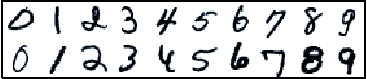
\includegraphics[width=0.48\columnwidth]{../figures/many_rbm_cond_witness_peaks}
  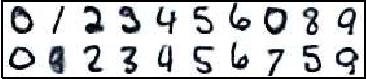
\includegraphics[width=0.48\columnwidth]{../figures/many_rbm_cond_witness_troughs}
\end{center}

Aside from some mistakes, the overrepresented digits appear fuzzy.
But maybe we just need to go deeper and use a DBN?

\begin{center}
  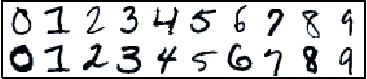
\includegraphics[width=0.48\columnwidth]{../figures/dbn_ft_cond_witness_peaks}
  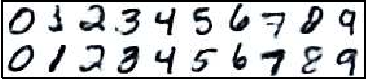
\includegraphics[width=0.48\columnwidth]{../figures/dbn_ft_cond_witness_troughs}
\end{center}

Here the overrepresented digits appear to have entire sections faded out.
The extra layers do not appear to have removed the fuzziness, it has just become more correlated.

%Note well, these overrepresented digits are not outliers, they are digits that are consistently produced by the models.

\vspace{0.5\baselineskip}

\mysection{A test of local heteroscedasticity}

\vspace{0.5\baselineskip}

Shown below left is some data and the fit of a Gaussian process regression model.
On the right is the witness function after performing a kernel two sample test.

\begin{center}
  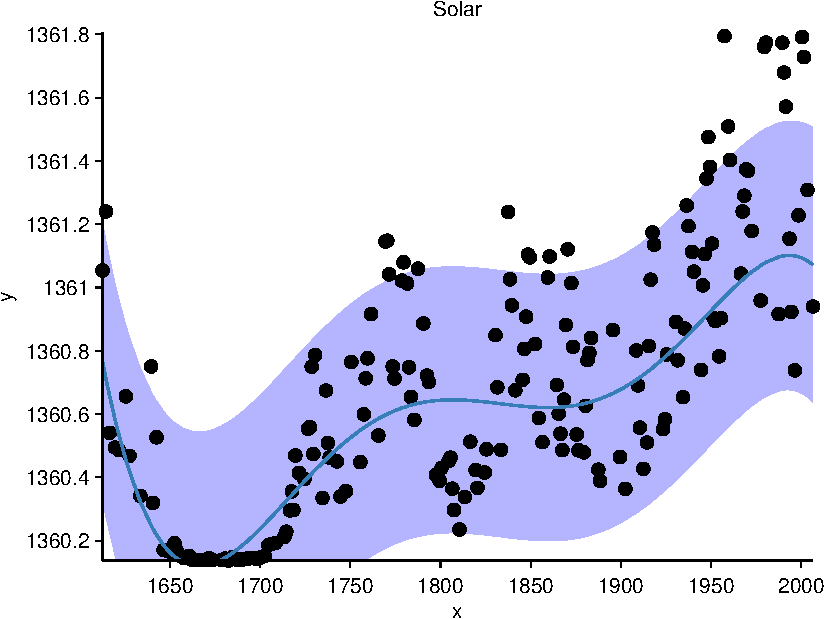
\includegraphics[width=0.48\columnwidth]{../figures/solar-data}
  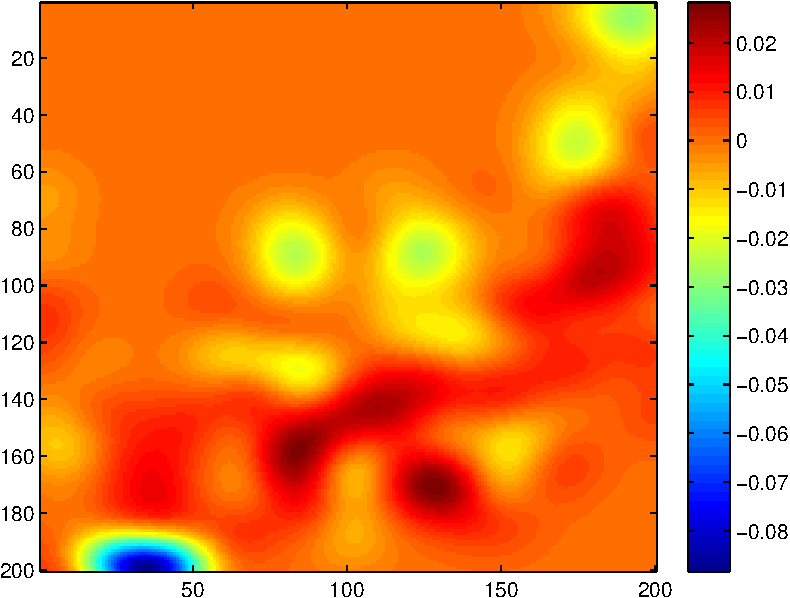
\includegraphics[width=0.48\columnwidth]{../figures/solar-witness}
\end{center}

The test identifies that something strange is happening at the bottom left.
Indeed, this is a region of very low data variability that the homoscedastic model fit to it cannot represent.

\vspace{0.5\baselineskip}

\mysection{Discussion and conclusion}

\vspace{0.5\baselineskip}

Did we answer our central question of how to choose a statistic for model criticism?
Not really, but these methods are interesting since one can specify a statistic in high level terms e.g.\ `smooth function' rather than specifying an equation.
You might also be wondering what happened to statistical power, or why the answer to misspecified models is not just to try fitting ever larger ones.
There's not quite enough space to write my thoughts here; talk to me or read the last chapter of my thesis!

\vspace{0.5\baselineskip}

We end by encouraging you to try model criticism methods and ask yourself, \textbf{Do you know how the model you are currently working with most misrepresents the data it is attempting to model?}

\end{multicols}

\end{poster}

\end{document}

